%===================================================================================
\section{Interfaces del subsistema: Gestión de tareas}

\subsection{CU20 Configuración de tareas}
{
\justify
\color{blue}{\textbf{Objetivo}}
}

%------------------------------------------------------------------
\justify
Permite al Lider de proyecto configurar las tareas que se realizaranen el proyecto, poder visuizaras en un diagrama de gantt y gestionar los avances atraves de un diagrama de representacion de avances por tareas.
%------------------------------------------------------------------
{
\justify
\color{blue}{\textbf{Diseño}}
}
%-------------------------------------------------------------------------------
\justify
En la figura \ref{fig:IU20} se muestra la pantalla, en donde permíte al Lider de proyecto configurar las tareas que se realizaranen el proyecto, poder visuizaras en un diagrama de gantt y gestionar los avances atraves de un diagrama de representacion de avances por tareas.

\begin{figure}[htb]
\centering
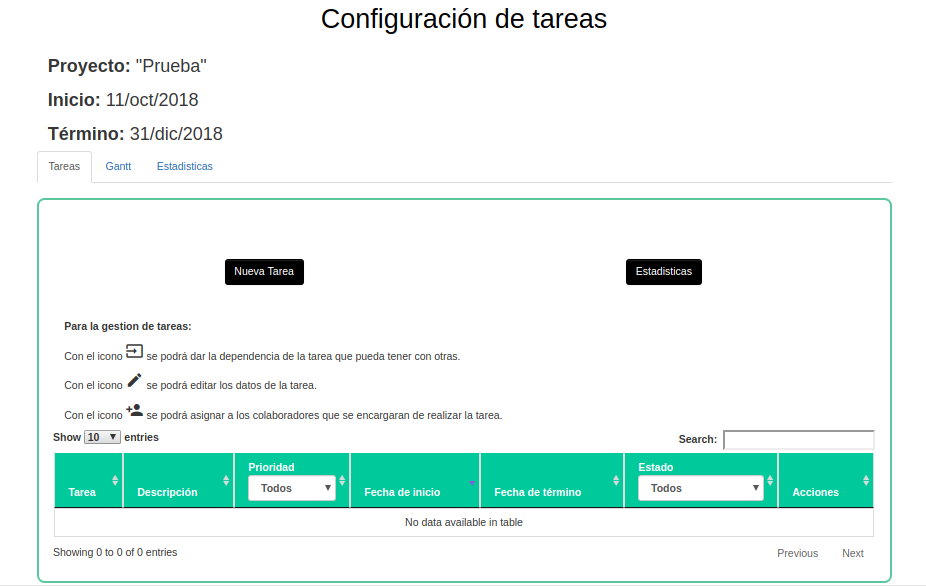
\includegraphics[width=0.8\textwidth]{./images/cu20-configurar-tareas.png}
\caption{Configuración de tareas.} \label{fig:IU20}
\end{figure}